\begin{figure*}[ht!]
\begin{center}% note that \centering uses less vspace...
\resizebox{2\columnwidth}{!}{%
\begin{tabular}{lllll}


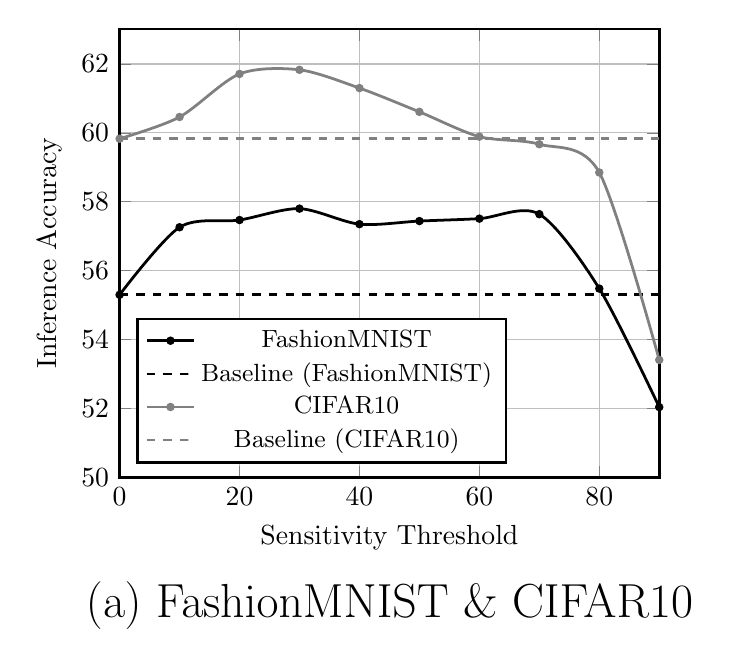
\begin{tikzpicture}
\begin{axis}[
title={(a) FashionMNIST \& CIFAR10},
title style={at={(0.5,0)},anchor=north,yshift=-40, font=\LARGE},
legend style={font=\small},
legend pos =  south west,
line width=1.0pt,
mark size=1.0pt,
ymin=50,
xmin=0,
xmax=90,
legend entries={FashionMNIST, Baseline (FashionMNIST), CIFAR10, Baseline (CIFAR10)},
ylabel={Inference Accuracy},
xlabel={Sensitivity Threshold},
% extra x ticks={1,10,...,400},
% extra y ticks={0,0.5,...,10},
% extra y tick labels={},
% extra x tick labels={},
% extra x tick style={grid=major},
% extra y tick style={grid=major},
grid=major
]
\addplot[
    color=black,
    solid,
    mark=*,
    mark options={solid},
    smooth
    ]
    coordinates {
    (0,55.30)(10,57.26)(20,57.47)(30,57.80)(40,57.35)(50,57.44)(60,57.51)(70,57.64)(80,55.48)(90,52.04)
      };
\addplot[
    color=black,
    dashed,
    smooth
    ]
    coordinates {
    (0,55.30)(10,55.30)(20,55.30)(30,55.30)(40,55.30)(50,55.30)(60,55.30)(70,55.30)(80,55.30)(90,55.30)
      };
\addplot[
    color=gray,
    solid,
    mark=*,
    mark options={solid},
    smooth
    ]
    coordinates {
    (0,59.83)(10,60.46)(20,61.71)(30,61.83)(40,61.30)(50,60.61)(60,59.89)(70,59.67)(80,58.85)(90,53.41)
      };
\addplot[
    color=gray,
    dashed,
    smooth
    ]
    coordinates {
    (0,59.83)(10,59.83)(20,59.83)(30,59.83)(40,59.83)(50,59.83)(60,59.83)(70,59.83)(80,59.83)(90,59.83)
      };
\end{axis}
\end{tikzpicture} &


%
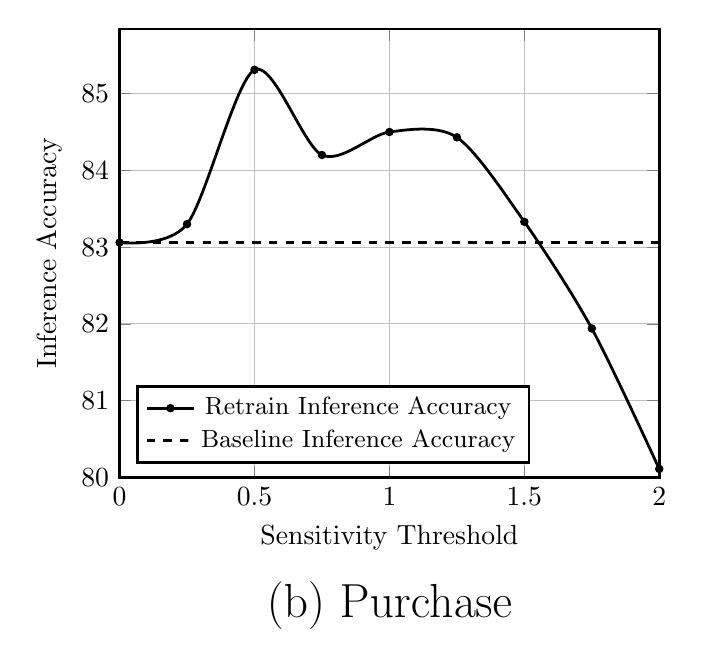
\begin{tikzpicture}
\begin{axis}[
title={(b) Purchase},
title style={at={(0.5,0)},anchor=north,yshift=-40, font=\LARGE},
legend style={font=\small},
legend pos =  south west,
line width=1.0pt,
mark size=1.0pt,
ymin=80,
xmin=0,
xmax=2,
legend entries={Retrain Inference Accuracy, Baseline Inference Accuracy},
ylabel={Inference Accuracy},
xlabel={Sensitivity Threshold},
grid=major
]
\addplot[
    color=black,
    solid,
    mark=*,
    mark options={solid},
    smooth
    ]
    coordinates {
    (0,83.06)(0.25,83.30)(0.5,85.31)(0.75,84.20)(1,84.50)(1.25,84.43)(1.5,83.33)(1.75,81.94)(2,80.11)
      };
\addplot[
    color=black,
    dashed,
    smooth
    ]
    coordinates {
    (0,83.06)(0.25,83.06)(0.5,83.06)(0.75,83.06)(1,83.06)(1.25,83.06)(1.5,83.06)(1.75,83.06)(2,83.06)
      };

\end{axis}
\end{tikzpicture} &
%
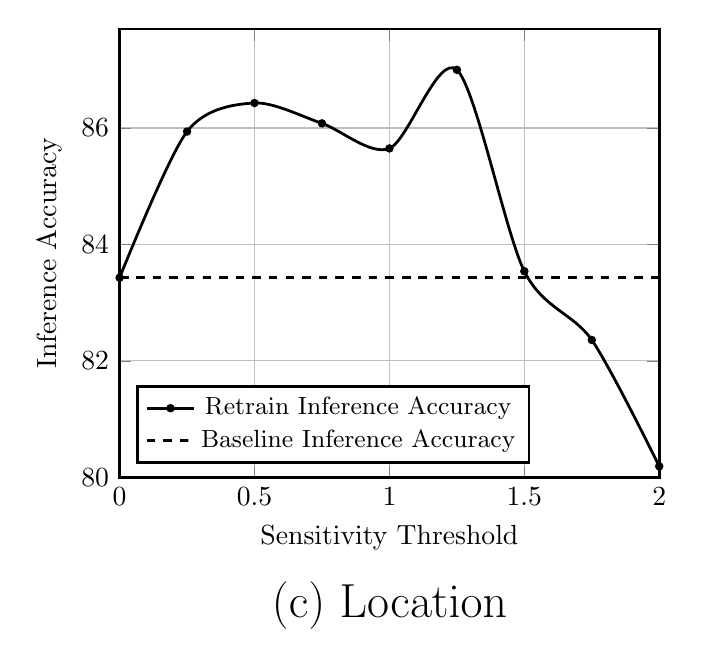
\begin{tikzpicture}
\begin{axis}[
title={(c) Location},
title style={at={(0.5,0)},anchor=north,yshift=-40, font=\LARGE},
legend style={font=\small},
legend pos =  south west,
line width=1.0pt,
mark size=1.0pt,
ymin=80,
xmin=0,
xmax=2,
legend entries={Retrain Inference Accuracy, Baseline Inference Accuracy},
ylabel={Inference Accuracy},
xlabel={Sensitivity Threshold},
grid=major
]
\addplot[
    color=black,
    solid,
    mark=*,
    mark options={solid},
    smooth
    ]
    coordinates {
    (0,83.43)(0.25,85.94)(0.5,86.43)(0.75,86.08)(1,85.65)(1.25,87.00)(1.5,83.54)(1.75,82.36)(2,80.19)
      };
\addplot[
    color=black,
    dashed,
    smooth
    ]
    coordinates {
    (0,83.43)(0.25,83.43)(0.5,83.43)(0.75,83.43)(1,83.43)(1.25,83.43)(1.5,83.43)(1.75,83.43)(2,83.43)
      };

\end{axis}
\end{tikzpicture}


\end{tabular}
}
\caption{Retraining the pruned model restores the original prediction accuracy but leads to more information memorized as well as more information leakage.}
%\caption{\underline{Retraining the pruned model leaks more information}. As required by the pruning algorithm, the pruned model is retrained to restore the original accuracy. This increases the information stored per parameter, i.e, each parameter is required to memorize more information about the training data to achieve original accuracy. This additional memorization by model parameters results in leaking more information.}
\label{fig:retrain}
\end{center}
\end{figure*}
